%% sections/03_methodology.tex
\section{Methodology}
\label{sec:methodology}

Section~\ref{subsec:problem_formulation} states the setting, threat model, and assumptions. Section~\ref{subsec:theory} gives two scoped observations that motivate server-side reference scoring. Section~\ref{subsec:framework} defines FU-Alignment, and Sections~\ref{subsec:client_side} and~\ref{subsec:governance} describe the shared client stack and audit ledger.

% =========================================================================
\subsection{Setting, Threat Model and Assumptions}
\label{subsec:problem_formulation}

\paragraph{Federated graph learning}
Let $\mathcal{G} = (\mathcal{V}, \mathcal{E}, X, A)$ be an attributed graph partitioned across $K$ clients. Client $k$ holds a subgraph $\mathcal{G}_k = (\mathcal{V}_k, \mathcal{E}_k, X_k, A_k)$ with disjoint node sets, and edges between different clients are not observed by anyone. Each node $v$ has a binary label $Y(v)$ and a binary sensitive attribute $S(v)$, such as gender or race. The clients jointly train the parameters $\theta \in \RR^P$ of a graph neural network. Fairness is measured by the demographic parity disparity
\begin{equation}
\label{eq:dpd_def}
\dpd(\theta) = \left| P(\hat{Y}=1 \mid S=0) - P(\hat{Y}=1 \mid S=1) \right|,
\end{equation}
which a federation may require to satisfy
\begin{equation}
\label{eq:dpd_constraint}
\dpd(\theta) \le \tau
\end{equation}
for a tolerance $\tau \ge 0$. We also report the equal opportunity disparity
\begin{equation}
\label{eq:eod_def}
\eod(\theta) = \left| P(\hat{Y}=1 \mid Y=1, S=0) - P(\hat{Y}=1 \mid Y=1, S=1) \right|.
\end{equation}

\paragraph{Design goals}
An aggregation rule for this setting should (i) prevent a client from gaining weight through anything it declares about itself, (ii) limit poisoned-update influence in specified threat models, and (iii) preserve useful predictive performance in benign runs. Section~\ref{sec:experiments} evaluates these goals without assuming that one rule dominates under every attack.

\paragraph{Threat model}
Following Kerckhoffs' principle, the adversary knows the architecture, losses, and aggregation rule. It controls $f < K/2$ clients, which may send arbitrary updates and arbitrary reports. Section~\ref{subsec:setup} evaluates three access schedules: sustained poisoning, intermittent poisoning that alternates honest and poisoning phases, and reference evasion that optimises an update against a surrogate of the server reference. Availability attacks, Sybil participation, and contamination of the server holdout remain outside the threat model.

\paragraph{Assumptions on the server holdout}
The rule of Section~\ref{subsec:framework} relies on a small labelled holdout graph $\Droot$ kept by the server. We make three assumptions about it; the adaptive-access study probes adaptive access but does not exhaustively test violations of these assumptions:
\begin{enumerate}[leftmargin=*, label=\textbf{A\arabic*}]
    \item \textbf{Clean.} The labels and sensitive attributes of $\Droot$ are correct. In a cross-silo federation such a set can be an audit sample held by a regulator or curated by the consortium. FLTrust assumes a clean root dataset at the server~\citep{cao2021fltrust}, and GuardFed likewise keeps a small share of real labelled data there~\citep{li2025guardfed}; we additionally need the sensitive attribute of these nodes.
    \item \textbf{Confidential.} Clients can read neither $\Droot$ nor the reference gradient computed on it.
    \item \textbf{Representative.} $\Droot$ approximates the target population well enough for its task and fairness gradients to be useful references.
\end{enumerate}
We do not consider cryptographic attestation, trusted hardware at every client, or incentive mechanisms that would make the reports themselves trustworthy. The rule below requires none of them at the clients, and the server may keep its holdout in a trusted execution environment to support A2.

% =========================================================================
\subsection{Analytical Motivation}
\label{subsec:theory}

Two observations motivate a reference computed by the server: report-free weights are invariant to report falsification, and update similarity alone need not reveal a small orthogonal perturbation. Neither observation establishes general robustness.

\paragraph{Rules that read reports}
\label{subsubsec:theory_immunity}

The weights of a report-reading rule depend on numbers that clients choose. The converse is immediate and worth stating because Section~\ref{subsec:rq1_audit} verifies it directly.

\begin{remark}[Rules that read no report]
\label{prop:syntactic_immunity}
If the weights depend only on the client updates and on quantities computed by the server, that is, $\bm{w} = \mathcal{F}(\{\Delta_k\}_{k=1}^K, \gtarg)$, then
\begin{equation}
\label{eq:zero_deriv}
\frac{\partial w_k}{\partial \widehat{\dpd}_j} \equiv 0 \qquad \forall\, k, j \in [K],
\end{equation}
so no falsified report can change them. FLTrust and the rule of Section~\ref{subsec:framework} have this property by construction, and CGSV reads no disparity report. It is necessary but not sufficient for robustness: a reference derived from the client updates, as in CGSV, can still be moved by a coordinated group of clients, and a task-only server reference, as in FLTrust, carries no information about fairness.
\end{remark}

A natural repair for a report-reading rule is to privatise the reports. Each client then releases its two group means $\mu_{k,a}$, the mean soft prediction of group $a$, with Gaussian noise:
\begin{equation}
\label{eq:scalar_dp}
\tilde{\mu}_{k,a} = \mu_{k,a} + \xi_{k,a}, \quad \xi_{k,a} \sim \mathcal{N}\left(0, \sigma_k^2\right), \quad \sigma_k = z\,\Delta_{\bm{\mu},k},
\end{equation}
where $\Delta_{\bm{\mu},k} = \sqrt{1/n_{k,0}^2 + 1/n_{k,1}^2}$ is the $\ell_2$ sensitivity of $(\mu_{k,0}, \mu_{k,1})$ and $z$ is the smallest noise multiplier for which R\'enyi accounting~\citep{mironov2017renyi} over all $R \cdot E$ releases of a run gives $(\epsilon, \delta) = (8, 10^{-5})$; for example, $z = 4.94$ for $R = 20$, $E = 3$. The reported disparity is $\widetilde{\dpd}_k = |\tilde{\mu}_{k,0} - \tilde{\mu}_{k,1}|$. Section~S2 of the Supplementary Information (ESM~1) shows that this repair has two defects. Because the reported disparity is an absolute value, Gaussian noise biases it upwards even when a client satisfies demographic parity, and the bias accumulates across clients instead of cancelling. In addition, a two-point Le~Cam argument shows that a single round of $K$ reports cannot reliably separate clients with disparity at most $\tau/2$ from clients with disparity at least $3\tau/2$ unless $\tau\sqrt{K}$ is large relative to the effective noise level. Both statements concern one round of independent Gaussian releases and the report channel only; they motivate a reference that the server computes itself rather than a general impossibility result for private fairness mechanisms.

Our earlier rule BFWA enforces the constraint by dual steps on such reports. Its response in Section~\ref{subsec:rq1_audit} identifies sensitivity of that reporting channel rather than a defect in its honest-report optimization.

\paragraph{Detectors that compare updates}
\label{subsubsec:theory_subspace}

Rules that read no report, such as Krum or FLAME, judge each update by its distance to the others. A perturbation that changes only fairness can stay close to the benign updates under such a distance.

\begin{proposition}[Cosine distance cannot separate fairness-only perturbations]
\label{prop:subspace_blindness}
Let $\RR^P = \mathcal{S}_{\mathrm{task}} \oplus \mathcal{S}_{\mathrm{fair}}$ with $\mathcal{S}_{\mathrm{fair}} = \mathcal{S}_{\mathrm{task}}^\perp$, and consider a detector that thresholds the cosine distance $\mathcal{D}_{\mathrm{cos}}(u_i, u_j) = 1 - \frac{\ip{u_i}{u_j}}{\norm{u_i}_2 \norm{u_j}_2}$ at $\rho_{\mathrm{thresh}} \in (0, 1)$. Then for any benign update $u_{\mathrm{benign}} \in \mathcal{S}_{\mathrm{task}}$ and any $\delta_{\mathrm{fair}} \in \mathcal{S}_{\mathrm{fair}}$ with $\norm{\delta_{\mathrm{fair}}}_2 < \sqrt{\rho_{\mathrm{thresh}}/(1 - \rho_{\mathrm{thresh}})}\, \norm{u_{\mathrm{benign}}}_2$, the update $u_{\mathrm{adv}} = u_{\mathrm{benign}} + \delta_{\mathrm{fair}}$ satisfies
\begin{equation}
\label{eq:blindness_dist}
\mathcal{D}_{\mathrm{cos}}(u_{\mathrm{adv}}, u_{\mathrm{benign}}) \le \frac{\norm{\delta_{\mathrm{fair}}}_2^2}{\norm{u_{\mathrm{benign}}}_2^2 + \norm{\delta_{\mathrm{fair}}}_2^2} < \rho_{\mathrm{thresh}},
\end{equation}
so the detector cannot separate $u_{\mathrm{adv}}$ from $u_{\mathrm{benign}}$.
\end{proposition}
\begin{proof}
Because $\ip{u_{\mathrm{benign}}}{\delta_{\mathrm{fair}}} = 0$,
\begin{align*}
\mathcal{D}_{\mathrm{cos}}(u_{\mathrm{adv}}, u_{\mathrm{benign}})
&= 1 - \frac{\norm{u_{\mathrm{benign}}}_2^2}{\sqrt{\norm{u_{\mathrm{benign}}}_2^2 + \norm{\delta_{\mathrm{fair}}}_2^2}\, \norm{u_{\mathrm{benign}}}_2} \\
&= 1 - \left(1 + \frac{\norm{\delta_{\mathrm{fair}}}_2^2}{\norm{u_{\mathrm{benign}}}_2^2}\right)^{-1/2}.
\end{align*}
The inequality $1 - 1/\sqrt{1+x} \le x/(1+x)$ gives the first inequality of Eq.~\eqref{eq:blindness_dist}, and the condition on $\norm{\delta_{\mathrm{fair}}}_2$ is equivalent to $x/(1+x) < \rho_{\mathrm{thresh}}$ for $x = \norm{\delta_{\mathrm{fair}}}_2^2/\norm{u_{\mathrm{benign}}}_2^2$.
\end{proof}

\begin{remark}[Scope]
\label{rem:subspace_blindness_scope}
The proposition says that such a perturbation cannot be detected, not how much weight it receives or how much disparity it adds; Section~\ref{sec:experiments} measures both. That benign updates lie, at least approximately, in $\mathcal{S}_{\mathrm{task}}$ is an idealisation that we did not measure, and $\mathcal{S}_{\mathrm{fair}}$ is defined geometrically, without fairness semantics of its own. The result applies to detectors that threshold cosine distance, such as the clustering in FLAME, and not to Krum and Multi-Krum, which use Euclidean distances.
\end{remark}

% =========================================================================
\subsection{FU-Alignment: Scoring Updates Against a Server Reference}
\label{subsec:framework}

FU-Alignment replaces the reports by a reference that only the server can compute (Figure~\ref{fig:pipeline}). In words: the server shrinks every update to norm at most $C$, measures to first order how much the update would lower the server's loss on its holdout, keeps a running average of that measurement for each client, and averages the clipped updates with weights proportional to the positive part of the running average.

\begin{figure}[t]
\centering
\IfFileExists{figures/fig_pipeline.pdf}{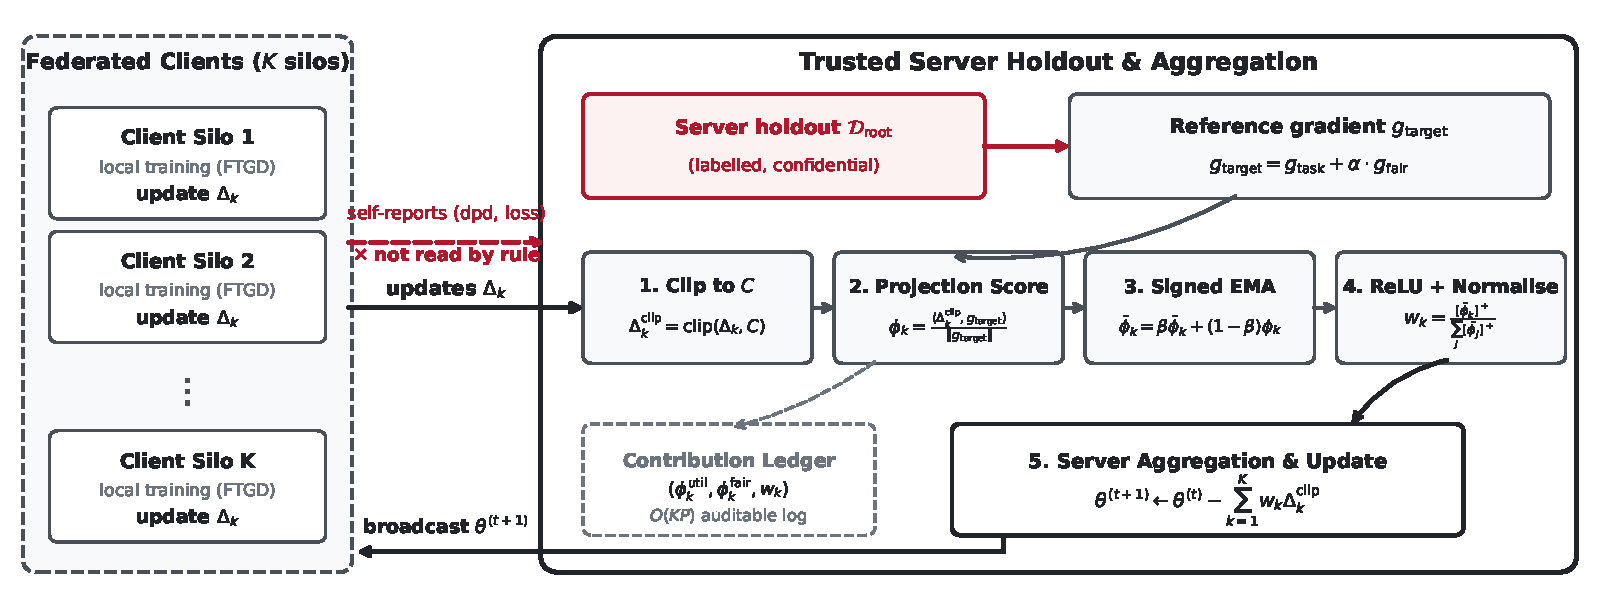
\includegraphics[width=\linewidth]{figures/fig_pipeline.pdf}}{\fbox{\parbox{0.9\linewidth}{\centering Figure in preparation.}}}
\caption{\textbf{FU-Alignment.} Clients send only their updates; the reports that report-reading rules depend on are not read. The server computes a reference gradient on its own holdout graph, clips each update, scores it by its projection onto the reference, smooths the scores over rounds, and averages the clipped updates with weights proportional to the positive part of the smoothed scores. The two parts of each score are logged for audit.}
\label{fig:pipeline}
\end{figure}

\paragraph{Server reference}
Before the clients are formed, the server sets aside up to 200 nodes of the label-stratified validation split, and never more than half of it, as its holdout $\Droot$ (125 nodes on German Credit and 200 on the larger graphs). No client owns these nodes, and no edge connects them to a client subgraph. In round $t$ the server evaluates two gradients on $\Droot$ at the current global model:
\begin{equation}
\label{eq:srv_grads}
\begin{gathered}
\gtask^{\mathrm{srv}} = \nabla_\theta \mathcal{L}_{\mathrm{task}}(\theta^{(t)}; \Droot), \qquad \gfair^{\mathrm{srv}} = \nabla_\theta \mathcal{L}^{\mathrm{srv}}_{\mathrm{fair}}(\theta^{(t)}; \Droot), \\
\mathcal{L}^{\mathrm{srv}}_{\mathrm{fair}} = (\mu_0^{\mathrm{srv}} - \mu_1^{\mathrm{srv}})^2,
\end{gathered}
\end{equation}
where $\mu_a^{\mathrm{srv}}$ is the mean soft prediction for group $a$ on $\Droot$. The squared gap is differentiable at zero, and the server computes it on its own data without noise. The reference combines the two gradients with a fixed weight $\alpha \ge 0$:
\begin{equation}
\label{eq:gtarg_def}
\gtarg^{(t)} = \gtask^{\mathrm{srv}} + \alpha\, \gfair^{\mathrm{srv}}.
\end{equation}
The fairness term tilts the reference towards lower disparity on the holdout. It does not filter clients by itself, and at $\alpha = 0.1$ its measured effect on allocation is negligible (Section~\ref{subsec:rq2_rq3_efficacy}).

\paragraph{Scoring and aggregation}
Each client update $\Delta_k^{(t)} = \theta^{(t)} - \theta_k^{(t)}$ is first clipped to norm $C$,
\begin{equation}
\label{eq:clip_pre_score}
\Delta_k^{\mathrm{clip}(t)} = \Delta_k^{(t)} \cdot \min\left(1, \frac{C}{\norm{\Delta_k^{(t)}}_2}\right),
\end{equation}
and then scored by its projection onto the reference,
\begin{equation}
\label{eq:score_raw}
\varphi_k^{(t)} = \frac{\ip{\Delta_k^{\mathrm{clip}(t)}}{\gtarg^{(t)}}}{\norm{\gtarg^{(t)}}_2}.
\end{equation}
An update that would raise the server's holdout objective, such as a sign-flipped one, receives a negative score. The signed scores are smoothed over rounds,
\begin{equation}
\label{eq:ema_smooth}
\bar{\varphi}_k^{(0)} = \varphi_k^{(0)}, \qquad \bar{\varphi}_k^{(t)} = \beta\, \bar{\varphi}_k^{(t-1)} + (1-\beta)\, \varphi_k^{(t)} \quad (t \ge 1),
\end{equation}
and only then rectified and normalised,
\begin{equation}
\label{eq:weights_simplex}
w_k^{(t)} = \frac{\ReLU(\bar{\varphi}_k^{(t)}) \cdot \mathbb{I}(\norm{\Delta_k^{(t)}} > 0)}{\sum_{j=1}^K \ReLU(\bar{\varphi}_j^{(t)}) \cdot \mathbb{I}(\norm{\Delta_j^{(t)}} > 0)},
\end{equation}
with uniform weights over the clients with a non-zero update if no smoothed score is positive. The global model moves by the weighted clipped updates:
\begin{equation}
\label{eq:model_update}
\theta^{(t+1)} = \theta^{(t)} - \sum_{k=1}^K w_k^{(t)} \Delta_k^{\mathrm{clip}(t)}.
\end{equation}
The canonical FU-Alignment cells use $\alpha = 0.1$, $\beta = 0.9$, and $C = 10$; campaign manifests record any campaign-specific variation.

\paragraph{Design rationale}
Each element answers a weakness identified in Section~\ref{subsec:theory}; Sections~\ref{subsec:rq4_boundary} and~\ref{subsec:rq2_rq3_efficacy} evaluate the resulting rule as a whole.
\begin{enumerate}[leftmargin=*, label=(\roman*)]
    \item \textbf{The reference does not depend on the clients.} Its task and fairness signals are computed on server-held data.
    \item \textbf{The score bounds magnitude and keeps direction.} Clipping before scoring caps what a single update can contribute to its score and to the aggregate (Proposition~\ref{prop:bounded_influence}), while the projection retains its component along the reference. The factorial ablation in Section~\ref{subsec:rq2_rq3_efficacy} shows that replacing clipping by rescaling increases adversarial weight.
    \item \textbf{The score remembers its sign.} Because the signed score is smoothed before it is rectified, a client that turns against the reference loses its weight within a bounded number of rounds (Proposition~\ref{prop:bounded_influence}), and a client that has opposed the reference must point towards it for several rounds before it regains weight.
\end{enumerate}

Table~\ref{tab:rule_comparison} sets these choices against FLTrust and GuardFed, the two server-anchored rules closest to ours.

\begin{table}[t]
\centering
\footnotesize
\caption{\textbf{FU-Alignment against the closest server-anchored rules.} The three rules all score clients against data held by the server; they differ in what the score measures, how update magnitude is handled, and whether scores carry memory. FLTrust and GuardFed as described in~\citep{cao2021fltrust, li2025guardfed}.}
\label{tab:rule_comparison}
\setlength{\tabcolsep}{4pt}
\begin{tabular}{p{0.17\linewidth}p{0.24\linewidth}p{0.26\linewidth}p{0.24\linewidth}}
\toprule
 & \textbf{FLTrust} & \textbf{GuardFed} & \textbf{FU-Alignment} \\
\midrule
Reference & server model update on root data & update of a reference model trained on server and synthetic data with fairness reweighting & task gradient plus $\alpha$ times a fairness gradient on the holdout \\
Client score & ReLU of the cosine with the reference & ReLU of the cosine, times $e^{-\tau_{\mathrm{G}} g_k}$, where $g_k$ is the equal-opportunity gap of the client model & projection of the clipped update onto the reference \\
Update magnitude & every update rescaled to the reference norm & not modified & clipped to norm $C$ \\
Memory & none & none & EMA of the signed score, before rectification \\
Weights & proportional to the score & uniform over clients whose score exceeds $\Gamma_{\mathrm{G}}$ & proportional to the positive part of the smoothed score \\
Server work per round & one update on root data and $K$ cosines & a reference update, $K$ cosines and $K$ model evaluations & two gradients on the holdout and $K$ inner products \\
\bottomrule
\end{tabular}
\end{table}

\begin{proposition}[Bounded influence]
\label{prop:bounded_influence}
Let the weights be given by Eq.~\eqref{eq:weights_simplex}, including the uniform fallback, and the global update by Eq.~\eqref{eq:model_update}.
\begin{enumerate}[leftmargin=*, label=(\roman*)]
    \item Whatever finite updates the clients send, $\norm{\theta^{(t+1)} - \theta^{(t)}}_2 \le C$.
    \item Suppose that client $k$ has $\varphi_k^{(t)} \le -m$ for some $m > 0$ and all $t \ge t_0 \ge 1$. Then $\bar{\varphi}_k^{(t)} \le 0$, and hence $w_k^{(t)} = 0$ whenever the fallback is not used, for all $t \ge t_0 + s - 1$ with
    \begin{equation}
    \label{eq:bounded_rounds}
    s = \left\lceil \frac{\log\left( (C + m)/m \right)}{\log(1/\beta)} \right\rceil .
    \end{equation}
\end{enumerate}
\end{proposition}
\begin{proof}
(i) In both branches the weights are non-negative and sum to one, and $\norm{\Delta_k^{\mathrm{clip}(t)}}_2 \le C$, so $\norm{\sum_k w_k^{(t)} \Delta_k^{\mathrm{clip}(t)}}_2 \le \sum_k w_k^{(t)} \norm{\Delta_k^{\mathrm{clip}(t)}}_2 \le C$.
(ii) By the Cauchy--Schwarz inequality $|\varphi_k^{(t)}| \le \norm{\Delta_k^{\mathrm{clip}(t)}}_2 \le C$ for every $t$, and therefore $\bar{\varphi}_k^{(t)} \le C$, since it is a convex combination of scores. Unrolling Eq.~\eqref{eq:ema_smooth} for $n \ge 1$ rounds from $t_0 - 1$ gives
$\bar{\varphi}_k^{(t_0 - 1 + n)} = \beta^{n} \bar{\varphi}_k^{(t_0-1)} + (1-\beta) \sum_{j=0}^{n-1} \beta^{j} \varphi_k^{(t_0 - 1 + n - j)} \le \beta^{n} C - m (1 - \beta^{n})$,
which is non-positive as soon as $\beta^{n} \le m/(C+m)$, that is, for all $n \ge s$. A non-positive smoothed score has zero rectified value, so the numerator of Eq.~\eqref{eq:weights_simplex} vanishes.
\end{proof}

Part (i) means that no update, however large, can move the global model by more than $C$ in one round. Part (ii) means that a client that persistently opposes the reference loses its weight after at most $s$ rounds. If it opposes the reference in every round from the first one, Eq.~\eqref{eq:ema_smooth} gives $\bar{\varphi}_k^{(t)} \le -m$ in every round by induction, so its weight is zero from the start whenever the fallback is not used; the delay of $s$ rounds applies only to a client that first builds up positive history, and for small $m$ it can exceed the length of our runs. Neither part bounds the weight of an adversary whose update is aligned with the reference; Section~\ref{sec:experiments} measures that case.

\paragraph{Server requirements and cost}
The server needs a holdout of at most $200$ labelled nodes with their sensitive attribute. In each round it evaluates two gradients on the holdout, clips the $K$ updates and computes $K$ inner products, which costs $O(KP)$ in addition to the two gradient evaluations. The clients run standard local training and need to send only their updates.

\begin{algorithm}[t]
\footnotesize
\caption{One round of FU-Alignment}
\label{alg:trustfedgnn}
\begin{algorithmic}[1]
\REQUIRE Global model $\theta^{(t)}$, holdout $\Droot$, smoothed scores $\bar{\varphi}^{(t-1)}$, $\alpha = 0.1$, $\beta = 0.9$, $C = 10$.
\ENSURE $\theta^{(t+1)}$, $\bar{\varphi}^{(t)}$ and the ledger entries of round $t$.
\STATE Compute $\gtask^{\mathrm{srv}}$ and $\gfair^{\mathrm{srv}}$ on $\Droot$ and set $\gtarg^{(t)} \gets \gtask^{\mathrm{srv}} + \alpha \gfair^{\mathrm{srv}}$ \hfill Eqs.~\eqref{eq:srv_grads}--\eqref{eq:gtarg_def}
\STATE Broadcast $\theta^{(t)}$; each client $k$ trains locally (Section~\ref{subsec:client_side}) and returns $\Delta_k^{(t)}$
\FOR{each client $k \in [K]$}
    \STATE $\Delta_k^{\mathrm{clip}(t)} \gets \Delta_k^{(t)} \cdot \min(1, C / \norm{\Delta_k^{(t)}}_2)$ \hfill Eq.~\eqref{eq:clip_pre_score}
    \STATE $\varphi_k^{(t)} \gets \ip{\Delta_k^{\mathrm{clip}(t)}}{\gtarg^{(t)}} / \norm{\gtarg^{(t)}}_2$ \hfill Eq.~\eqref{eq:score_raw}
    \STATE $\bar{\varphi}_k^{(t)} \gets \varphi_k^{(t)}$ if $t = 0$, else $\beta \bar{\varphi}_k^{(t-1)} + (1-\beta) \varphi_k^{(t)}$ \hfill Eq.~\eqref{eq:ema_smooth}
\ENDFOR
\STATE Compute $w^{(t)}$ by Eq.~\eqref{eq:weights_simplex}, with the uniform fallback over clients with $\Delta_k^{(t)} \ne \mathbf{0}$
\STATE $\theta^{(t+1)} \gets \theta^{(t)} - \sum_k w_k^{(t)} \Delta_k^{\mathrm{clip}(t)}$ \hfill Eq.~\eqref{eq:model_update}
\STATE Log $\langle t, k, w_k^{(t)}, \varphi_k^{\mathrm{util}}, \varphi_k^{\mathrm{fair}} \rangle$ for every $k$ \hfill Eq.~\eqref{eq:audit_tuple}
\end{algorithmic}
\end{algorithm}

% =========================================================================
\subsection{Client-Side Training Stack}
\label{subsec:client_side}

To isolate the server-side aggregation mechanism, all methods evaluated in this paper use a common local training stack that adapts the FSER and FTGD ideas from our prior work~\citep{dang2026fedfairgnn}. These fixed client-side components are not claimed as contributions of this study. TrustFedGNN's aggregation path consumes model updates and server-computed reference signals without using client-reported fairness or performance statistics.

The local backbone is a two-layer GAT~\citep{velickovic2017graph} with hidden dimension $64$, batch normalisation, and residual connections, combined with fairness-sensitive edge reweighting (FSER), which initially attenuates inter-group edges by a factor $\gamma_{\mathrm{init}} = 0.5$. Local training adapts fair targeted gradient descent (FTGD). Each client computes a task gradient and the gradient of a fairness loss $\mathcal{L}_{\mathrm{fair}} = |\mu_{k,0} - \mu_{k,1}|$ built from its group means; when report privatisation is enabled, the released means $\tilde{\mu}_{k,a}$ of Eq.~\eqref{eq:scalar_dp} replace them and are computed by a forward pass that does not take $S$ as input:
\begin{equation}
\label{eq:local_grads}
g_{k,\mathrm{task}} = \nabla_\theta \mathcal{L}_{\mathrm{task}}(\theta; \mathcal{G}_k), \qquad g_{k,\mathrm{fair}} = \nabla_\theta \mathcal{L}_{\mathrm{fair}}(\theta; \mathcal{G}_k).
\end{equation}
It removes from the task gradient its component along the fairness gradient,
\begin{equation}
\label{eq:ftgd_proj}
g_k^{\perp} = \begin{cases}
g_{k,\mathrm{task}} - \dfrac{\ip{g_{k,\mathrm{task}}}{g_{k,\mathrm{fair}}}}{\norm{g_{k,\mathrm{fair}}}^2}\, g_{k,\mathrm{fair}}, & \norm{g_{k,\mathrm{fair}}} \ge 10^{-8}, \\
g_{k,\mathrm{task}}, & \text{otherwise},
\end{cases}
\end{equation}
so that $\ip{g_k^{\perp}}{g_{k,\mathrm{fair}}} = 0$, and steps along
\begin{equation}
\label{eq:ftgd_update_step}
u_k = g_k^{\perp} + g_{k,\mathrm{fair}}.
\end{equation}

To run every rule under a common protocol, each client also exports a report containing its training-set size, validation AUC, loss, disparity, and equal opportunity gap; when privatisation is enabled, the reported disparity is the privatised one. FU-Alignment and FLTrust never read this report; CGSV reads only the sample count in a fallback branch, while the report exists for the rules that read it. Privatisation therefore protects a channel that FU-Alignment does not use.

% =========================================================================
\subsection{Contribution Ledger}
\label{subsec:governance}

Because the reference is a sum of two gradients, each score splits exactly into a utility part and a fairness part.

\begin{proposition}[Linear decomposition]
\label{prop:linear_shapley}
For every client and round,
\begin{equation}
\label{eq:linear_decomp}
\varphi_k^{(t)} = \varphi_k^{\mathrm{util}} + \varphi_k^{\mathrm{fair}}, \qquad
\varphi_k^{\mathrm{util}} = \frac{\ip{\Delta_k^{\mathrm{clip}(t)}}{\gtask^{\mathrm{srv}}}}{\norm{\gtarg^{(t)}}_2}, \quad
\varphi_k^{\mathrm{fair}} = \frac{\alpha \ip{\Delta_k^{\mathrm{clip}(t)}}{\gfair^{\mathrm{srv}}}}{\norm{\gtarg^{(t)}}_2},
\end{equation}
and both parts cost $O(KP)$ per round.
\end{proposition}
\begin{proof}
The inner product is linear in its second argument and $\gtarg^{(t)} = \gtask^{\mathrm{srv}} + \alpha \gfair^{\mathrm{srv}}$; dividing by the common normaliser preserves the identity.
\end{proof}

In every round the server appends
\begin{equation}
\label{eq:audit_tuple}
\mathcal{T}_k^{(t)} = \left\langle t, k, w_k^{(t)}, \varphi_k^{\mathrm{util}}, \varphi_k^{\mathrm{fair}} \right\rangle
\end{equation}
to a round log, which records how much of each client's score came from utility and how much from fairness. The implementation stores both parts before the division by $\norm{\gtarg^{(t)}}_2$, which leaves their ratio unchanged. By construction of Eq.~\eqref{eq:weights_simplex}, the weights lie on the probability simplex and a client that sends a zero update receives zero weight. The decomposition is a first-order attribution and does not approximate Shapley values.
